\section{Binary Symmetric Channel}
\subsection{Gallagher-A decoder}
\begin{frame}{Gallagher’s Decoding Algorithm A}
\;\;\;\;\;\;Consider a ($d_v, d_c$) regular
LDPC code over the Binary Symmetric Channel (BSC). The BSC
is completely specified by a parameter p, the crossover probability.
The channel behaves as illustrated in below Figure. The correct bit is
transmitted with probability 1-p and a bit flip occurs with probability
p. Hence I = O = ±1. For this decoding algorithm $\mathcal{M}$ is also equal
to ±1. This is called hard-decision decoding 
\begin{exampleblock}{Binary Symmetric Channel}
\begin{figure}
			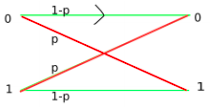
\includegraphics[width=8cm, height=4cm]{BSC/bsc.png}
			\label{bsc}
\end{figure}
\end{exampleblock}

\end{frame}

\begin{frame}{Gallagher's A (cont...)}
$\bullet$ $V^{0}(y) = y$  Variable nodes simply pass the received value as
their first message\\~\\
$\bullet$ $C^{(l)}(m_1, . . . , m_{d_c-1}) = m_1m_2 . . . m_{d_c-1}.$ For all l, the message from check node c to variable node v is the product of the messages received by c from all it’s neighbors except v. This makes perfect sense, since if the messages c received were indeed the correct values of the code word bit, then the parity check represented by c would only be satisfied if v were the product of the messages. Note that mod 2 addition corresponds
to multiplication after the identification of 0 with 1 and 1 with -1 respectively.\\~\\
$\bullet$ $V^{(l)}(y, m_1, . . . , m_{d_v-1}) = -y$ if all\;\; $ m_i = -y$ and y otherwise. For all subsequent rounds, v still sends the received value, y as its message to c unless there is unanimous agreement amongst all checks except c, that v participates in.
\end{frame}

\begin{frame}{Gallagher's A (cont...)}
\;\;\;\;\;\;\;\; This decoder is clearly sub-optimal since it does not even depend on the channel parameter p. Nonetheless, experimental simulations and theoretical analysis show that it is not too bad. We will analyze the asymptotic behavior of this decoder later in this section. in below Figures 
shows this algorithm in action. The code being used is a (3, 6) regular LDPC code. The all ones vector +\,+\,+\,+\,+\,+\,+\,+\,+\,+\, was transmitted. Due to channel noise, the received vector is +\,+\,+\,-\,+\,+\,+\,+\,+\,-\,. The first set of messages sent, Figure a, therefore correspond to the received values. The second set of messages, Figure b, were sent by the check nodes to the variable nodes. By 5 iterations, the algorithm converges to the vector -\,+\,-\,-\,-\,+\,-\,+\,+\,-\, which is indeed a valid code word but not the correct one. Hence this example serves to illustrate how message passing decoders can fail. Note that a high failure rate is expected since the block length is very small.\\~\\
following figures shows Gallagher’s algorithm A in action. R indicates the round number. The direction of arrows indicate the direction of message sent. Red corresponds to -1 and Green to 1    
\end{frame}
\begin{frame}{Gallagher's A (cont...)}
\begin{exampleblock}{Gallagher’s algorithm A in action}

\begin{figure}
			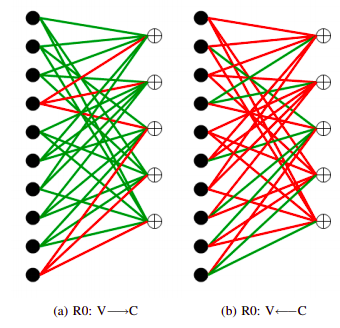
\includegraphics[width=6cm, height=3.3cm]{BSC/gallaghar fig 2a.png}
			\label{fig2a}
\end{figure}
\begin{figure}
			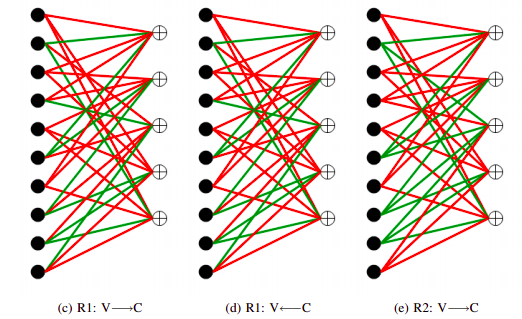
\includegraphics[width=8cm, height=3.3cm]{BSC/gallaghar fig 2b.png}
			\label{fig2b}
\end{figure}
\end{exampleblock}

\end{frame}

\subsection{Belief Propagation for BSC}
\begin{frame}{Belief Propagation for BSC}
$\bullet$ $V^{(0)}(y) = l_i$. Here $l_i$ is the log likelihood of the code word bit $x_i$ conditioned on the received bit $y_i$. The value depends on the channel model in use. For instance, consider the binary symmetric channel with crossover probability p. Then $y_i$ $\in$ \{-1, 1\}. Under the assumption of equiprobability, if the received code word was 1, then
 \begin{gather*}
     l_i = \log L(x_i/y_i = 1) = \log \frac{p}{1-p}
 \end{gather*} 
 otherwise 
 \begin{gather*}
     l_i = -\log\frac{p}{1-p}
 \end{gather*}

$\bullet$ $V^{(l)}(y, m_1, . . . , m_{d_v-1}) = l_i + $$\sum_{i=1}^{d_v-1} m_i$$ $ The reasoning behind this is that if $m_i$ are conditional log likelihoods of $x_i$, conditioned on independent random variables, then the
aggregate conditional would indeed by given by this equation
\end{frame}
\begin{frame}{Belief Propagation for BSC(cont...)}
\begin{gather*}
 C^{(l)}(m_1, . . . , m_{d_c-1})   = \log \frac{1 + \prod_{i=1}^{d_c-1} \tanh(m_i/2)}{1 - \prod_{i=1}^{d_c-1} \tanh(m_i/2)}
 \end{gather*}
$\bullet$  If the incoming messages are independent estimates of the log likelihood of $x_j$ , the neighbors of the check node computing the message excluding node xi, then the computed message $C^{(l)}$ correctly estimates the likelihood of $x_i$ conditioned on the the messages and the fact that the parity check represented by the check node is satisfied. \\~\\Consequently, under the independence assumption, the belief propagation algorithm correctly performs bit wise MAP decoding.
\end{frame}

\subsection{Results}
\begin{frame}
\begin{exampleblock}{Terminal output for Belief Propagation}
    \begin{figure}
		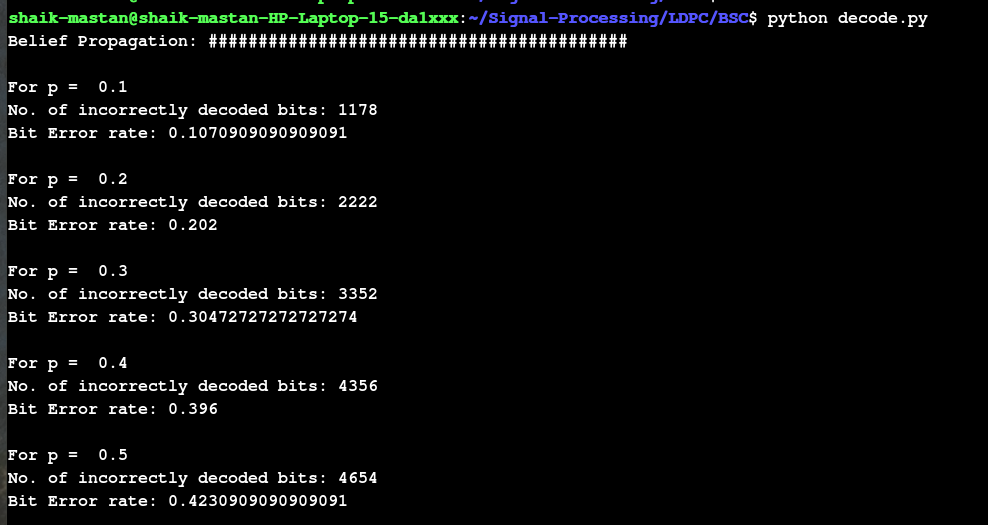
\includegraphics[width=\textwidth]{BSC/terminalBSC_1.png}
	\end{figure}
\end{exampleblock}
\end{frame}

\begin{frame}
\begin{exampleblock}{Terminal output for Gallagher-A}
    \begin{figure}
		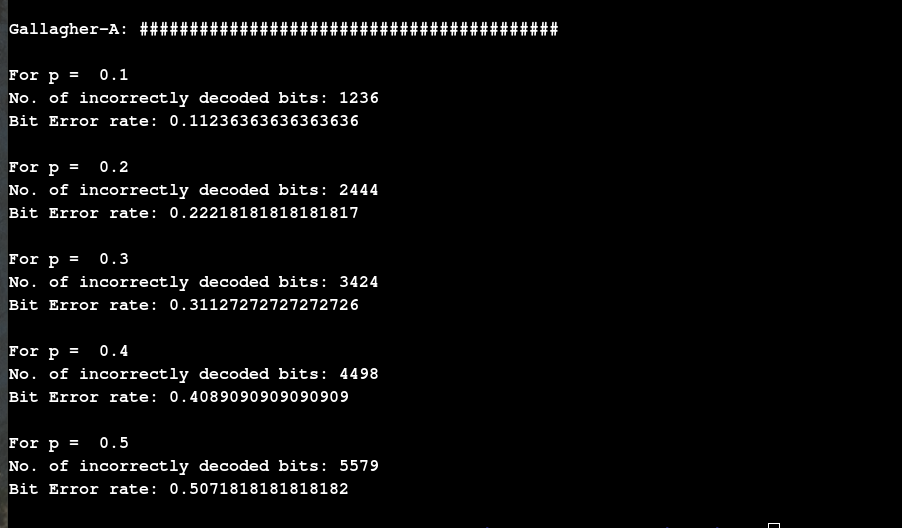
\includegraphics[width=\textwidth]{BSC/terminalBSC_2.png}
	\end{figure}
\end{exampleblock}
\end{frame}

\begin{frame}
\begin{exampleblock}{Comparison between the two decoders}
    \begin{figure}
		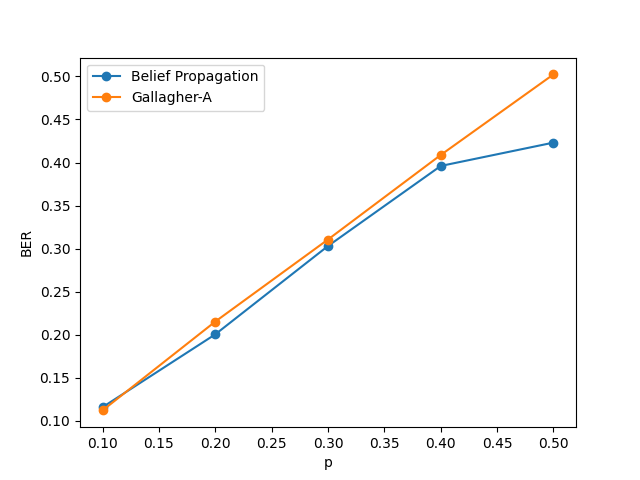
\includegraphics[width=0.9\textwidth]{BSC/BSC.png}
	\end{figure}
\end{exampleblock}

\end{frame}